\documentclass[bachelor_thesis]{subfiles}

\begin{document}
\chapter{Theoretical background} \label{chap:theory}
\section{Plasma Wakefield acceleration}
\Gls{pwfa} is a novel particle accelerator concept \cite{Chen1985} with the possibility to produce high accelerating electric fields (more than \qty{100}{\giga\volt/\m}). This allows for higher energy gains per meter
and thus several order of magnitude smaller accelerators, compared to conventional \gls{rf} accelerators.

\Gls{pwfa} works by sending a bunch of charged particles (also called drive beam or driver) with relativistic speed ($v_{beam}\approx c$) into a neutral plasma. Multiple sources are possible for this beam and will be further discussed in \autoref{chap:lpfwa}.
In this thesis, the beam consists of electrons but research on other species like positrons \cite{Gessner2016} is made as well. To be easily ionized, the plasma is often formed by light weight gases like lithium (or even hydrogen or helium in newer experiments \cite{Schoebel2022}), 
ionized either by the drive beam itself or a dedicated ionization laser.

When entering the plasma, the drive beam interacts with the plasma electrons, while the effect on the ions can be neglected at the time scale of the electron response. The electric field of the bunch pushes the electrons out of its way, comparable to a snowplow. 
This leaves an electron free cavity behind, starting from the center of the driver while the expelled electrons culminate at the borders of the cavity. As the ions are not moving, this cavity is positively charged, meaning it acts as an attractive force to the plasma electrons.
When being pulled back towards the center of the cavity, the electrons overshoot and produce another cavity. The result is electron oscillation, where multiple cavities form behind the beam as seen in \autoref{fig:pwfa}.

\begin{figure}
	\centering
	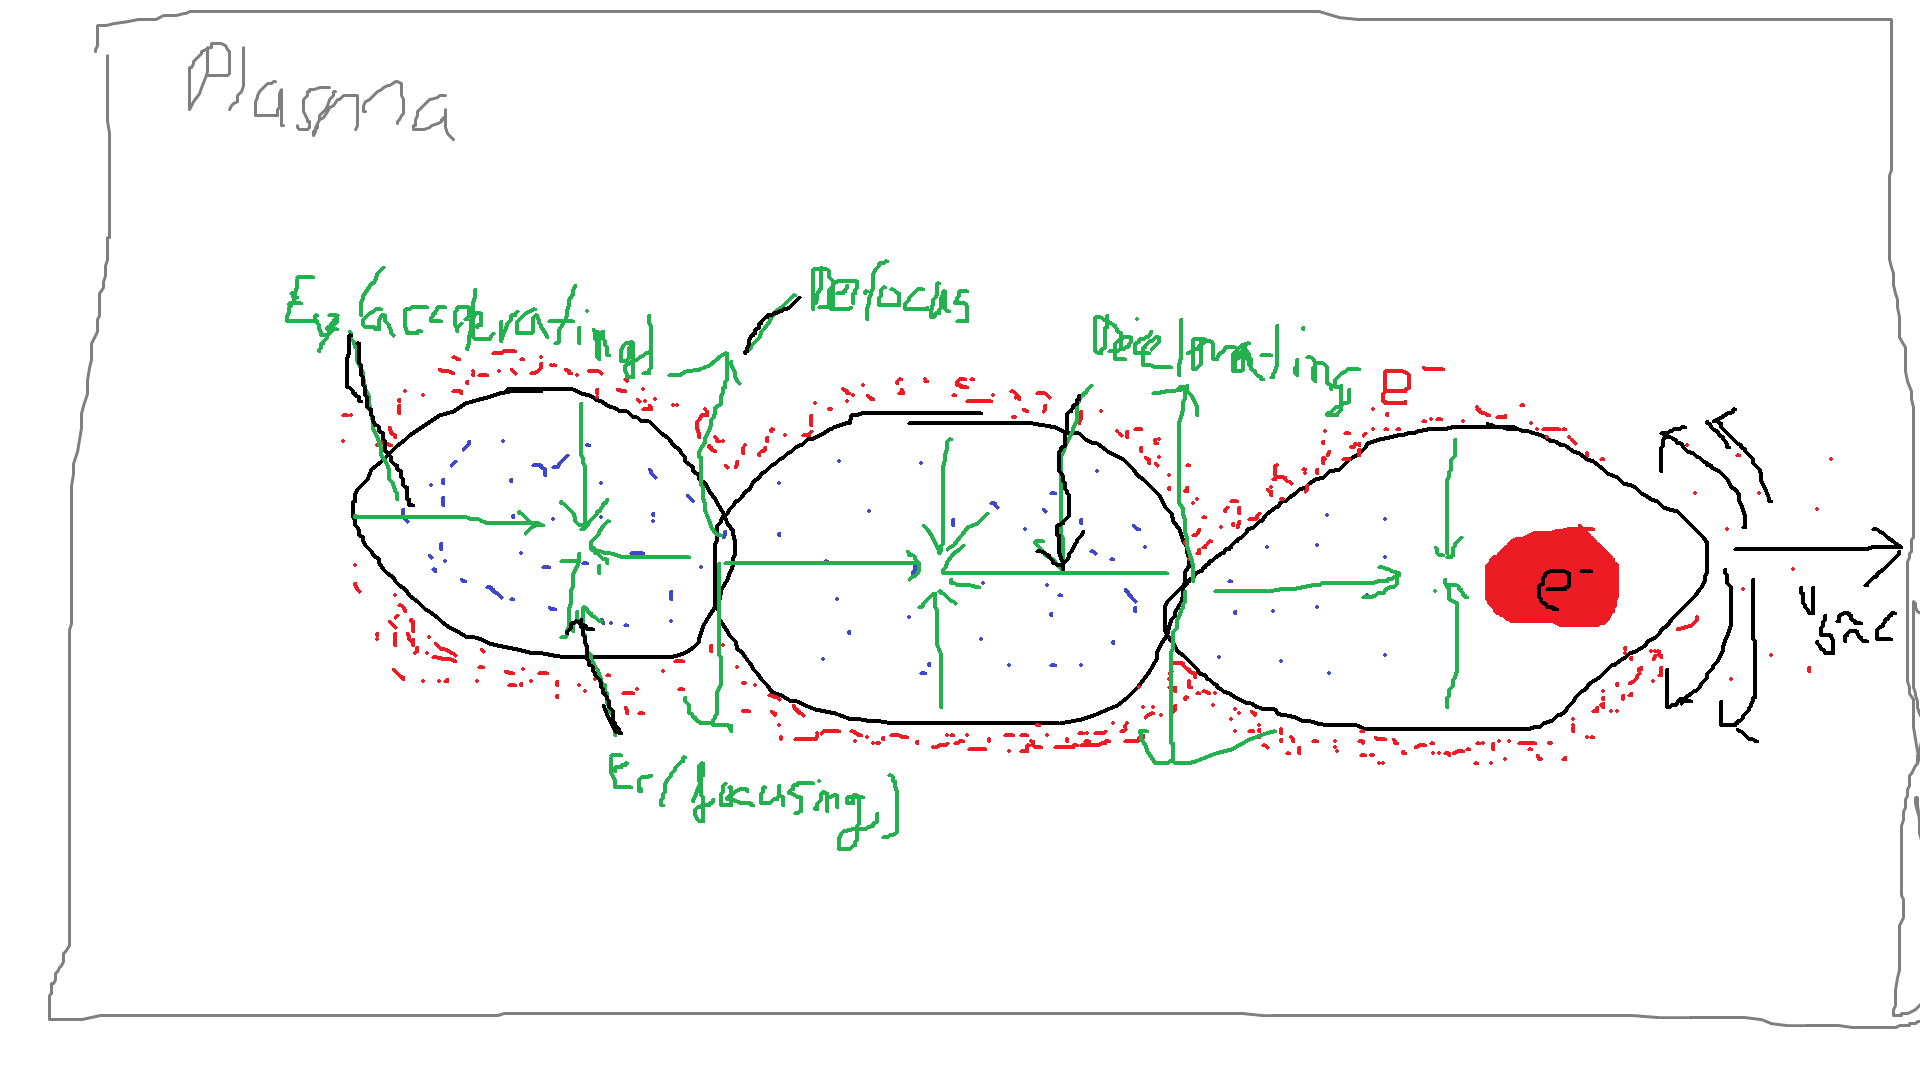
\includegraphics[scale=0.3]{pwfa.png}
	\caption{The blowout regime of a \gls{pwfa} stage with an electron driver at the front. Alternating accelerating/decelerating fields in transverse and focusing/defocusing fields in longitudinal direction form in the cavities. Inspired by \cite{Kurz2020}.}
	\label{fig:pwfa} \todo[inline]{placeholder, remake graphic}
\end{figure}

This train of cavities is called the wakefield. If the electron density in these cavities is several orders of magnitude smaller than in the rest of the plasma, this state is called the blowout regime, else only the linear regime.
When injecting a charged particle bunch, called the witness beam, into the wakefield, it sees fields acting from different directions due to the gradient towards the center of the positive cavity. 

For a witness beam in propagation direction, consisting of negative charged particles, the electric field accelerates towards the center of the cavity while decelerating when reaching its front half. 
Perpendicular to the direction of propagation are electric fields pointing towards the center and magnetic fields rotating, resulting in focusing of the witness beam. In contrast there are defocusing forces between the cavities, as the oscillating electrons are densest here.
When witness electrons are injected into the back of the cavity, they will be accelerated while the cavity itself moves at near light speed with the driver.
These accelerating forces peak when the wakefield is in the blowout regime, therefore achieving blowout as long as possible is a goal of \gls{pwfa}.

Near light speed, the velocity of the witness beam won't increase in a meaningful way. The witness electrons would therefore be trapped in the accelerating part of the cavity, resulting in a net increase of momentum and energy.

\subsection{LWFA driven PWFA} \label{chap:lpfwa}
For a long time, a big downside of \gls{pwfa} was the creation of the relativistic drive beams, as this would need kilometer long \gls{rf} accelerators as a preliminary stage. Recent research \cite{Kurz2021} investigated the potential of the so called \gls{lpwfa}.
Here, the witness bunch of a \gls{lwfa} was used as driver for the \gls{pwfa}, allowing for a very compact design.

\Gls{lwfa} is very similar to \gls{pwfa}. Instead of charged particles, here a laser is shot into a plasma to drive the wakefields, also generating hundreds of \unit{\giga\volt/\m} of accelerating fields.
The witness bunch can be accelerated to higher speeds than the speed of the laser in the plasma, resulting in dephasing, where the witness beam is fast enough to reach the center of the cavity and get decelerated. This limits the acceleration capabilities of the \gls{lwfa}
 but the resulting witness bunch can still be used as the driver for the \gls{pwfa}. As the driver here already moves roughly at light speed, dephasing is no problem. 

\begin{figure}
	\centering
	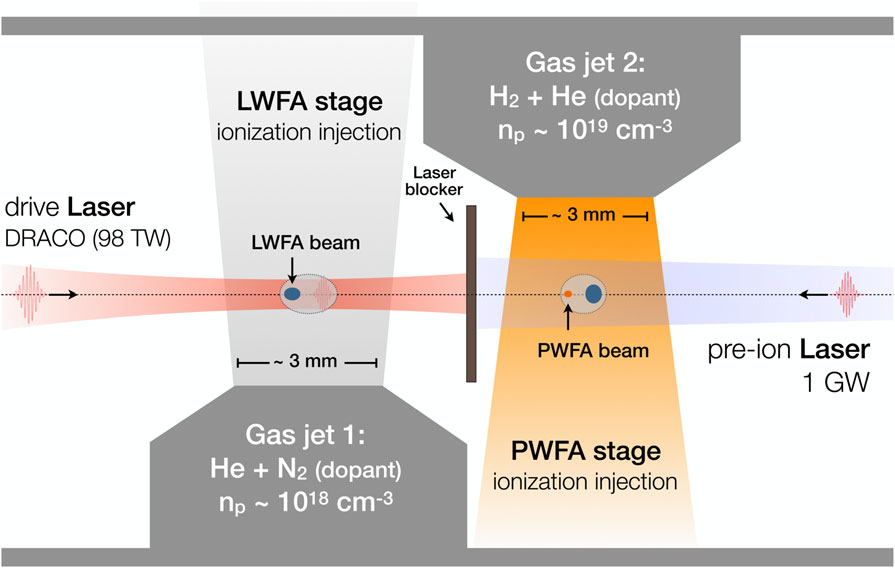
\includegraphics[scale=1.4]{lpwfa.png}
	\caption{Example for a \gls{lpwfa} setup. Taken from \cite{Ossa2019}}
	\label{fig:lpwfa} \todo[inline]{redo graphic}
\end{figure} 
Experimental setups for \gls{lpwfa} (see \autoref{fig:lpwfa}) consist of a laser initiating a \gls{lwfa} stage in a gas jet. 
Both, the accelerated witness bunch and the laser are leaving the jet into vacuum, where a metal foil is installed to block the laser and let only the particle beam through. 
Thus, only the witness bunch makes it to the next gas jet, serving as the driver for the \gls{pwfa} stage and accelerating injected electrons.
This hybrid scheme has the potential to advance the \gls{pwfa} research further and make it more accessible to small scale labs \cite{Kurz2021}.

\paragraph*{Peak energy}\hspace{0pt} \\
The energy with the highest charge density of driver particles is called peak energy. In experiment, it is an important measurement as it provides the beam charge of a witness beam leaving a \gls{lwfa} stage \cite{Schoebel2022}.
The peak energy of the driver is assumed to stay constant during a \gls{pwfa} stage, therefore information about the driver before entering the \gls{pwfa} can be obtained in a \gls{lpwfa}.

\autoref{chap:E_shift} will discuss evidence, that the peak energy is sinking during the \gls{pwfa} stage, and the assumption of constant peak energy therefore can only be made for high uncertainty measurements.


\section{PIConGPU}
To simulate complex driver-plasma interactions efficiently, the \acrfull{pic}-model is often chosen. There are many different code implementations, often developed to innovate with new techniques. For this thesis PIConGPU \cite{PIConGPU2013, PICRepo} is used, 
a relativistic \gls{pic}-code, which specializes in parallelization of the computational steps. Therefor it is designed to work on GPUs instead of CPUs. We will start with an introduction to the \gls{pic} method in general in \autoref{chap:pic}.
In the following subsection, we discuss further how certain inputs and outputs are handled in PIConGPU.

\subsection{Particle-in-cell model} \label{chap:pic}
\Gls{pic}-code models particles in a simulation box, generally described as a distribution function $f_s(\vec{x}, \vec{p}, t)$ of time $t$, position $\vec{x}$ and momentum $\vec{p}$ for every particle species $s$ \cite{PICRepo, Derouillat2017}.
This distribution must now satisfy the collisionless Boltzmann equation, also called Vlasov equation\cite{Vlasov1968}, see \autoref{equ:boltz}.

\begin{equation}
	\frac{\mathrm{d}f_s}{\mathrm{d}t}=\frac{\partial f_s}{\partial t} + \frac{\partial \vec{x}}{\partial t} \frac{\partial f_s}{\partial \vec{x}} + \frac{\partial \vec{p}}{\partial t} \frac{\partial f_s}{\partial \vec{p}} = 0
	\label{equ:boltz}
\end{equation}
Using the Nabla-Operator and the derivatives of $\vec{x}$ and $\vec{p}$, we get \autoref{equ:vlasov} with the Lorentz factor $\gamma$, the species mass $m_s$ and the Lorentz Force $\vec{F}_L$, see \autoref{equ:lorentz}.

\begin{equation}
	\partial_t f_s + \frac{\vec{p}}{m_s \gamma} \vec{\nabla}_{\vec{x}} f_s + \vec{F}_L \vec{\nabla}_{\vec{p}} f_s = 0
	\label{equ:vlasov}
\end{equation}

\begin{equation}
	\vec{F}_L=q_s\left(\vec{E}+\vec{v}\times\vec{B}\right)
	\label{equ:lorentz}
\end{equation}

To be a self-consistent set of electro-magnetic equations, the Maxwell equations (see \autoref{equ:maxwell}) need to be fulfilled by our $\vec{E}$- and $\vec{B}$-fields. Here $\rho_s$ and $\vec{J}_s$ are the charge and current density for a given species $s$.

\begin{equation}
\begin{aligned}
	\vec{\nabla}\cdotp\vec{E}  &= \frac{1}{\epsilon_0}\sum_s \rho_s 									\\
	\vec{\nabla}\cdotp\vec{B}  &= 0 														\\
	\vec{\nabla}\times\vec{E} &= -\frac{\partial \vec{B}}{\partial t}									\\
	\vec{\nabla}\times\vec{B}&= \mu_0 \left(\sum_s \vec{J}_s + \epsilon_0 \frac{\partial \vec{E}}{\partial t}\right)	
\end{aligned}
\label{equ:maxwell}
\end{equation}

The \gls{pic} model now makes several simplifications, so these requirements can be implemented.
At first, the time needs to be discretized into timesteps with length $\Delta t$ after which our distribution is updated. The equation system above must then be broken down into a system of computations, which will be processed every timestep.
This system is often called the \gls{pic}-cycle \cite{Huebl2019}, which can be seen in \autoref{fig:cycle}.

\begin{figure}
	\centering
	\resizebox{0.8\textwidth}{!}{%% Creator: Matplotlib, PGF backend
%%
%% To include the figure in your LaTeX document, write
%%   \input{<filename>.pgf}
%%
%% Make sure the required packages are loaded in your preamble
%%   \usepackage{pgf}
%%
%% Also ensure that all the required font packages are loaded; for instance,
%% the lmodern package is sometimes necessary when using math font.
%%   \usepackage{lmodern}
%%
%% Figures using additional raster images can only be included by \input if
%% they are in the same directory as the main LaTeX file. For loading figures
%% from other directories you can use the `import` package
%%   \usepackage{import}
%%
%% and then include the figures with
%%   \import{<path to file>}{<filename>.pgf}
%%
%% Matplotlib used the following preamble
%%
\begingroup%
\makeatletter%
\begin{pgfpicture}%
\pgfpathrectangle{\pgfpointorigin}{\pgfqpoint{6.400000in}{4.500000in}}%
\pgfusepath{use as bounding box, clip}%
\begin{pgfscope}%
\pgfsetbuttcap%
\pgfsetmiterjoin%
\pgfsetlinewidth{0.000000pt}%
\definecolor{currentstroke}{rgb}{1.000000,1.000000,1.000000}%
\pgfsetstrokecolor{currentstroke}%
\pgfsetstrokeopacity{0.000000}%
\pgfsetdash{}{0pt}%
\pgfpathmoveto{\pgfqpoint{0.000000in}{0.000000in}}%
\pgfpathlineto{\pgfqpoint{6.400000in}{0.000000in}}%
\pgfpathlineto{\pgfqpoint{6.400000in}{4.500000in}}%
\pgfpathlineto{\pgfqpoint{0.000000in}{4.500000in}}%
\pgfpathlineto{\pgfqpoint{0.000000in}{0.000000in}}%
\pgfpathclose%
\pgfusepath{}%
\end{pgfscope}%
\begin{pgfscope}%
\pgfpathrectangle{\pgfqpoint{0.150000in}{0.150000in}}{\pgfqpoint{6.100000in}{4.200000in}}%
\pgfusepath{clip}%
\pgfsetbuttcap%
\pgfsetmiterjoin%
\definecolor{currentfill}{rgb}{0.121569,0.466667,0.705882}%
\pgfsetfillcolor{currentfill}%
\pgfsetfillopacity{0.500000}%
\pgfsetlinewidth{1.003750pt}%
\definecolor{currentstroke}{rgb}{0.000000,0.000000,0.000000}%
\pgfsetstrokecolor{currentstroke}%
\pgfsetstrokeopacity{0.500000}%
\pgfsetdash{}{0pt}%
\pgfpathmoveto{\pgfqpoint{0.455000in}{0.234000in}}%
\pgfpathlineto{\pgfqpoint{2.590000in}{0.234000in}}%
\pgfpathquadraticcurveto{\pgfqpoint{2.773000in}{0.234000in}}{\pgfqpoint{2.773000in}{0.360000in}}%
\pgfpathlineto{\pgfqpoint{2.773000in}{1.830000in}}%
\pgfpathquadraticcurveto{\pgfqpoint{2.773000in}{1.956000in}}{\pgfqpoint{2.590000in}{1.956000in}}%
\pgfpathlineto{\pgfqpoint{0.455000in}{1.956000in}}%
\pgfpathquadraticcurveto{\pgfqpoint{0.272000in}{1.956000in}}{\pgfqpoint{0.272000in}{1.830000in}}%
\pgfpathlineto{\pgfqpoint{0.272000in}{0.360000in}}%
\pgfpathquadraticcurveto{\pgfqpoint{0.272000in}{0.234000in}}{\pgfqpoint{0.455000in}{0.234000in}}%
\pgfpathlineto{\pgfqpoint{0.455000in}{0.234000in}}%
\pgfpathclose%
\pgfusepath{stroke,fill}%
\end{pgfscope}%
\begin{pgfscope}%
\pgfpathrectangle{\pgfqpoint{0.150000in}{0.150000in}}{\pgfqpoint{6.100000in}{4.200000in}}%
\pgfusepath{clip}%
\pgfsetbuttcap%
\pgfsetmiterjoin%
\definecolor{currentfill}{rgb}{1.000000,0.498039,0.054902}%
\pgfsetfillcolor{currentfill}%
\pgfsetfillopacity{0.500000}%
\pgfsetlinewidth{2.007500pt}%
\definecolor{currentstroke}{rgb}{0.000000,0.000000,0.000000}%
\pgfsetstrokecolor{currentstroke}%
\pgfsetstrokeopacity{0.500000}%
\pgfsetdash{}{0pt}%
\pgfpathmoveto{\pgfqpoint{3.810000in}{2.544000in}}%
\pgfpathlineto{\pgfqpoint{5.945000in}{2.544000in}}%
\pgfpathquadraticcurveto{\pgfqpoint{6.128000in}{2.544000in}}{\pgfqpoint{6.128000in}{2.670000in}}%
\pgfpathlineto{\pgfqpoint{6.128000in}{4.140000in}}%
\pgfpathquadraticcurveto{\pgfqpoint{6.128000in}{4.266000in}}{\pgfqpoint{5.945000in}{4.266000in}}%
\pgfpathlineto{\pgfqpoint{3.810000in}{4.266000in}}%
\pgfpathquadraticcurveto{\pgfqpoint{3.627000in}{4.266000in}}{\pgfqpoint{3.627000in}{4.140000in}}%
\pgfpathlineto{\pgfqpoint{3.627000in}{2.670000in}}%
\pgfpathquadraticcurveto{\pgfqpoint{3.627000in}{2.544000in}}{\pgfqpoint{3.810000in}{2.544000in}}%
\pgfpathlineto{\pgfqpoint{3.810000in}{2.544000in}}%
\pgfpathclose%
\pgfusepath{stroke,fill}%
\end{pgfscope}%
\begin{pgfscope}%
\pgfpathrectangle{\pgfqpoint{0.150000in}{0.150000in}}{\pgfqpoint{6.100000in}{4.200000in}}%
\pgfusepath{clip}%
\pgfsetbuttcap%
\pgfsetmiterjoin%
\definecolor{currentfill}{rgb}{0.172549,0.627451,0.172549}%
\pgfsetfillcolor{currentfill}%
\pgfsetfillopacity{0.500000}%
\pgfsetlinewidth{2.007500pt}%
\definecolor{currentstroke}{rgb}{0.000000,0.000000,0.000000}%
\pgfsetstrokecolor{currentstroke}%
\pgfsetstrokeopacity{0.500000}%
\pgfsetdash{}{0pt}%
\pgfpathmoveto{\pgfqpoint{0.455000in}{2.544000in}}%
\pgfpathlineto{\pgfqpoint{2.590000in}{2.544000in}}%
\pgfpathquadraticcurveto{\pgfqpoint{2.773000in}{2.544000in}}{\pgfqpoint{2.773000in}{2.670000in}}%
\pgfpathlineto{\pgfqpoint{2.773000in}{4.140000in}}%
\pgfpathquadraticcurveto{\pgfqpoint{2.773000in}{4.266000in}}{\pgfqpoint{2.590000in}{4.266000in}}%
\pgfpathlineto{\pgfqpoint{0.455000in}{4.266000in}}%
\pgfpathquadraticcurveto{\pgfqpoint{0.272000in}{4.266000in}}{\pgfqpoint{0.272000in}{4.140000in}}%
\pgfpathlineto{\pgfqpoint{0.272000in}{2.670000in}}%
\pgfpathquadraticcurveto{\pgfqpoint{0.272000in}{2.544000in}}{\pgfqpoint{0.455000in}{2.544000in}}%
\pgfpathlineto{\pgfqpoint{0.455000in}{2.544000in}}%
\pgfpathclose%
\pgfusepath{stroke,fill}%
\end{pgfscope}%
\begin{pgfscope}%
\pgfpathrectangle{\pgfqpoint{0.150000in}{0.150000in}}{\pgfqpoint{6.100000in}{4.200000in}}%
\pgfusepath{clip}%
\pgfsetbuttcap%
\pgfsetmiterjoin%
\definecolor{currentfill}{rgb}{0.839216,0.152941,0.156863}%
\pgfsetfillcolor{currentfill}%
\pgfsetfillopacity{0.500000}%
\pgfsetlinewidth{2.007500pt}%
\definecolor{currentstroke}{rgb}{0.000000,0.000000,0.000000}%
\pgfsetstrokecolor{currentstroke}%
\pgfsetstrokeopacity{0.500000}%
\pgfsetdash{}{0pt}%
\pgfpathmoveto{\pgfqpoint{3.810000in}{0.234000in}}%
\pgfpathlineto{\pgfqpoint{5.945000in}{0.234000in}}%
\pgfpathquadraticcurveto{\pgfqpoint{6.128000in}{0.234000in}}{\pgfqpoint{6.128000in}{0.360000in}}%
\pgfpathlineto{\pgfqpoint{6.128000in}{1.830000in}}%
\pgfpathquadraticcurveto{\pgfqpoint{6.128000in}{1.956000in}}{\pgfqpoint{5.945000in}{1.956000in}}%
\pgfpathlineto{\pgfqpoint{3.810000in}{1.956000in}}%
\pgfpathquadraticcurveto{\pgfqpoint{3.627000in}{1.956000in}}{\pgfqpoint{3.627000in}{1.830000in}}%
\pgfpathlineto{\pgfqpoint{3.627000in}{0.360000in}}%
\pgfpathquadraticcurveto{\pgfqpoint{3.627000in}{0.234000in}}{\pgfqpoint{3.810000in}{0.234000in}}%
\pgfpathlineto{\pgfqpoint{3.810000in}{0.234000in}}%
\pgfpathclose%
\pgfusepath{stroke,fill}%
\end{pgfscope}%
\begin{pgfscope}%
\pgfsetroundcap%
\pgfsetroundjoin%
\definecolor{currentfill}{rgb}{0.000000,0.000000,0.000000}%
\pgfsetfillcolor{currentfill}%
\pgfsetlinewidth{1.204500pt}%
\definecolor{currentstroke}{rgb}{0.000000,0.000000,0.000000}%
\pgfsetstrokecolor{currentstroke}%
\pgfsetdash{}{0pt}%
\pgfpathmoveto{\pgfqpoint{4.598291in}{2.890316in}}%
\pgfpathquadraticcurveto{\pgfqpoint{4.822433in}{2.329962in}}{\pgfqpoint{4.654173in}{1.769323in}}%
\pgfpathlineto{\pgfqpoint{4.720686in}{1.749361in}}%
\pgfpathquadraticcurveto{\pgfqpoint{4.649164in}{1.680505in}}{\pgfqpoint{4.572500in}{1.620000in}}%
\pgfpathquadraticcurveto{\pgfqpoint{4.558759in}{1.716803in}}{\pgfqpoint{4.534448in}{1.805255in}}%
\pgfpathlineto{\pgfqpoint{4.600962in}{1.785293in}}%
\pgfpathquadraticcurveto{\pgfqpoint{4.763644in}{2.327346in}}{\pgfqpoint{4.546709in}{2.869684in}}%
\pgfpathlineto{\pgfqpoint{4.598291in}{2.890316in}}%
\pgfpathlineto{\pgfqpoint{4.598291in}{2.890316in}}%
\pgfpathclose%
\pgfusepath{stroke,fill}%
\end{pgfscope}%
\begin{pgfscope}%
\pgfsetroundcap%
\pgfsetroundjoin%
\definecolor{currentfill}{rgb}{0.000000,0.000000,0.000000}%
\pgfsetfillcolor{currentfill}%
\pgfsetlinewidth{1.204500pt}%
\definecolor{currentstroke}{rgb}{0.000000,0.000000,0.000000}%
\pgfsetstrokecolor{currentstroke}%
\pgfsetdash{}{0pt}%
\pgfpathmoveto{\pgfqpoint{1.801709in}{1.609684in}}%
\pgfpathquadraticcurveto{\pgfqpoint{1.577567in}{2.170038in}}{\pgfqpoint{1.745827in}{2.730677in}}%
\pgfpathlineto{\pgfqpoint{1.679314in}{2.750639in}}%
\pgfpathquadraticcurveto{\pgfqpoint{1.750836in}{2.819495in}}{\pgfqpoint{1.827500in}{2.880000in}}%
\pgfpathquadraticcurveto{\pgfqpoint{1.841241in}{2.783197in}}{\pgfqpoint{1.865552in}{2.694745in}}%
\pgfpathlineto{\pgfqpoint{1.799038in}{2.714707in}}%
\pgfpathquadraticcurveto{\pgfqpoint{1.636356in}{2.172654in}}{\pgfqpoint{1.853291in}{1.630316in}}%
\pgfpathlineto{\pgfqpoint{1.801709in}{1.609684in}}%
\pgfpathlineto{\pgfqpoint{1.801709in}{1.609684in}}%
\pgfpathclose%
\pgfusepath{stroke,fill}%
\end{pgfscope}%
\begin{pgfscope}%
\pgfsetroundcap%
\pgfsetroundjoin%
\definecolor{currentfill}{rgb}{0.000000,0.000000,0.000000}%
\pgfsetfillcolor{currentfill}%
\pgfsetlinewidth{1.204500pt}%
\definecolor{currentstroke}{rgb}{0.000000,0.000000,0.000000}%
\pgfsetstrokecolor{currentstroke}%
\pgfsetdash{}{0pt}%
\pgfpathmoveto{\pgfqpoint{3.820316in}{1.174209in}}%
\pgfpathquadraticcurveto{\pgfqpoint{3.280041in}{0.958099in}}{\pgfqpoint{2.739474in}{1.118540in}}%
\pgfpathlineto{\pgfqpoint{2.719714in}{1.051966in}}%
\pgfpathquadraticcurveto{\pgfqpoint{2.650534in}{1.123317in}}{\pgfqpoint{2.590000in}{1.200000in}}%
\pgfpathquadraticcurveto{\pgfqpoint{2.686844in}{1.213732in}}{\pgfqpoint{2.775040in}{1.238373in}}%
\pgfpathlineto{\pgfqpoint{2.755281in}{1.171799in}}%
\pgfpathquadraticcurveto{\pgfqpoint{3.277337in}{1.016852in}}{\pgfqpoint{3.799684in}{1.225791in}}%
\pgfpathlineto{\pgfqpoint{3.820316in}{1.174209in}}%
\pgfpathlineto{\pgfqpoint{3.820316in}{1.174209in}}%
\pgfpathclose%
\pgfusepath{stroke,fill}%
\end{pgfscope}%
\begin{pgfscope}%
\pgfsetroundcap%
\pgfsetroundjoin%
\definecolor{currentfill}{rgb}{0.000000,0.000000,0.000000}%
\pgfsetfillcolor{currentfill}%
\pgfsetlinewidth{1.204500pt}%
\definecolor{currentstroke}{rgb}{0.000000,0.000000,0.000000}%
\pgfsetstrokecolor{currentstroke}%
\pgfsetdash{}{0pt}%
\pgfpathmoveto{\pgfqpoint{2.579684in}{3.325791in}}%
\pgfpathquadraticcurveto{\pgfqpoint{3.119959in}{3.541901in}}{\pgfqpoint{3.660526in}{3.381460in}}%
\pgfpathlineto{\pgfqpoint{3.680286in}{3.448034in}}%
\pgfpathquadraticcurveto{\pgfqpoint{3.749466in}{3.376683in}}{\pgfqpoint{3.810000in}{3.300000in}}%
\pgfpathquadraticcurveto{\pgfqpoint{3.713156in}{3.286268in}}{\pgfqpoint{3.624960in}{3.261627in}}%
\pgfpathlineto{\pgfqpoint{3.644719in}{3.328201in}}%
\pgfpathquadraticcurveto{\pgfqpoint{3.122663in}{3.483148in}}{\pgfqpoint{2.600316in}{3.274209in}}%
\pgfpathlineto{\pgfqpoint{2.579684in}{3.325791in}}%
\pgfpathlineto{\pgfqpoint{2.579684in}{3.325791in}}%
\pgfpathclose%
\pgfusepath{stroke,fill}%
\end{pgfscope}%
\begin{pgfscope}%
\definecolor{textcolor}{rgb}{0.000000,0.000000,0.000000}%
\pgfsetstrokecolor{textcolor}%
\pgfsetfillcolor{textcolor}%
\pgftext[x=1.522500in,y=3.825000in,,]{\color{textcolor}\sffamily\fontsize{18.000000}{21.600000}\bfseries\selectfont Force Calculation}%
\end{pgfscope}%
\begin{pgfscope}%
\definecolor{textcolor}{rgb}{0.000000,0.000000,0.000000}%
\pgfsetstrokecolor{textcolor}%
\pgfsetfillcolor{textcolor}%
\pgftext[x=4.877500in,y=3.825000in,,]{\color{textcolor}\sffamily\fontsize{18.000000}{21.600000}\bfseries\selectfont Particle Push}%
\end{pgfscope}%
\begin{pgfscope}%
\definecolor{textcolor}{rgb}{0.000000,0.000000,0.000000}%
\pgfsetstrokecolor{textcolor}%
\pgfsetfillcolor{textcolor}%
\pgftext[x=4.877500in,y=1.410000in,,]{\color{textcolor}\sffamily\fontsize{18.000000}{21.600000}\bfseries\selectfont Current Deposition}%
\end{pgfscope}%
\begin{pgfscope}%
\definecolor{textcolor}{rgb}{0.000000,0.000000,0.000000}%
\pgfsetstrokecolor{textcolor}%
\pgfsetfillcolor{textcolor}%
\pgftext[x=1.522500in,y=1.410000in,,]{\color{textcolor}\sffamily\fontsize{18.000000}{21.600000}\bfseries\selectfont Field Evolution}%
\end{pgfscope}%
\begin{pgfscope}%
\definecolor{textcolor}{rgb}{0.000000,0.000000,0.000000}%
\pgfsetstrokecolor{textcolor}%
\pgfsetfillcolor{textcolor}%
\pgftext[x=1.522500in,y=3.300000in,,]{\color{textcolor}\sffamily\fontsize{14.000000}{16.800000}\selectfont \(\displaystyle \vec{F} = q \cdot \left( \vec{E} + \vec{v} \times \vec{B} \right)\)}%
\end{pgfscope}%
\begin{pgfscope}%
\definecolor{textcolor}{rgb}{0.000000,0.000000,0.000000}%
\pgfsetstrokecolor{textcolor}%
\pgfsetfillcolor{textcolor}%
\pgftext[x=4.877500in,y=3.300000in,,]{\color{textcolor}\sffamily\fontsize{14.000000}{16.800000}\selectfont \(\displaystyle \vec{p}_{i+1} = \vec{p}_{i} + \Delta t \cdot \vec{F} \)}%
\end{pgfscope}%
\begin{pgfscope}%
\definecolor{textcolor}{rgb}{0.000000,0.000000,0.000000}%
\pgfsetstrokecolor{textcolor}%
\pgfsetfillcolor{textcolor}%
\pgftext[x=4.877500in,y=0.948000in,,]{\color{textcolor}\sffamily\fontsize{14.000000}{16.800000}\selectfont \(\displaystyle \vec J = \int q \cdot \vec{v} \cdot f(\vec{r}, \vec{v}) \mathrm{d} V\)}%
\end{pgfscope}%
\begin{pgfscope}%
\definecolor{textcolor}{rgb}{0.000000,0.000000,0.000000}%
\pgfsetstrokecolor{textcolor}%
\pgfsetfillcolor{textcolor}%
\pgftext[x=1.522500in,y=0.570000in,,]{\color{textcolor}\sffamily\fontsize{14.000000}{16.800000}\selectfont \(\displaystyle  \frac{\partial \vec{E}}{\partial t}= c^2 \left( - \mu_0 \vec{j} + \vec{\nabla} \times \vec{B} \right)\)}%
\end{pgfscope}%
\begin{pgfscope}%
\definecolor{textcolor}{rgb}{0.000000,0.000000,0.000000}%
\pgfsetstrokecolor{textcolor}%
\pgfsetfillcolor{textcolor}%
\pgftext[x=1.522500in,y=0.948000in,,]{\color{textcolor}\sffamily\fontsize{14.000000}{16.800000}\selectfont \(\displaystyle  \frac{\partial \vec{B}}{\partial t}= - \vec{\nabla} \times \vec{E} \)}%
\end{pgfscope}%
\end{pgfpicture}%
\makeatother%
\endgroup%
}
	\caption{The \gls{pic}-cycle. In PIConGPU, every timestep starts with the force calculation. Figure taken from \cite{Pausch2019}}
	\label{fig:cycle}
\end{figure}

Instead of the complex high-dimensional distribution function $f_s(\vec{x}, \vec{p}, t)$, we look at a simulation box in 3 space dimensions and describe the distribution for a species as discrete macroparticles in this box \cite{Burau2010}.
The movement of these macro particles are then described by their position and momentum, the acceleration from the acting force depends on their set mass $m$, charge $q$ and weighting $w$.
The weighting is determined by the assignment density function which the macro particle represents and can also be seen as the number of real particles for each macro particle.
In this thesis, the assignment function of the driver particles is given by a piecewise quadratic spline.

At last, the fields need to be divided into the so-called Yee-grid \cite{Yee1966}, which can be seen in \autoref{fig:cell}. The corresponding fields are placed between the grid points, motivated by the fact that for the later described centered finite difference, 
the spatial derivative of the fields lies between these fields. At this points, the time derivatives are calculated and therefore the grid points positioned.

\begin{figure}
	\centering
	\resizebox{0.8\textwidth}{!}{%% Creator: Matplotlib, PGF backend
%%
%% To include the figure in your LaTeX document, write
%%   \input{<filename>.pgf}
%%
%% Make sure the required packages are loaded in your preamble
%%   \usepackage{pgf}
%%
%% Also ensure that all the required font packages are loaded; for instance,
%% the lmodern package is sometimes necessary when using math font.
%%   \usepackage{lmodern}
%%
%% Figures using additional raster images can only be included by \input if
%% they are in the same directory as the main LaTeX file. For loading figures
%% from other directories you can use the `import` package
%%   \usepackage{import}
%%
%% and then include the figures with
%%   \import{<path to file>}{<filename>.pgf}
%%
%% Matplotlib used the following preamble
%%
\begingroup%
\makeatletter%
\begin{pgfpicture}%
\pgfpathrectangle{\pgfpointorigin}{\pgfqpoint{6.400000in}{5.000000in}}%
\pgfusepath{use as bounding box, clip}%
\begin{pgfscope}%
\pgfsetbuttcap%
\pgfsetmiterjoin%
\pgfsetlinewidth{0.000000pt}%
\definecolor{currentstroke}{rgb}{1.000000,1.000000,1.000000}%
\pgfsetstrokecolor{currentstroke}%
\pgfsetstrokeopacity{0.000000}%
\pgfsetdash{}{0pt}%
\pgfpathmoveto{\pgfqpoint{0.000000in}{0.000000in}}%
\pgfpathlineto{\pgfqpoint{6.400000in}{0.000000in}}%
\pgfpathlineto{\pgfqpoint{6.400000in}{5.000000in}}%
\pgfpathlineto{\pgfqpoint{0.000000in}{5.000000in}}%
\pgfpathlineto{\pgfqpoint{0.000000in}{0.000000in}}%
\pgfpathclose%
\pgfusepath{}%
\end{pgfscope}%
\begin{pgfscope}%
\pgfpathrectangle{\pgfqpoint{0.000000in}{0.050000in}}{\pgfqpoint{6.400000in}{5.000000in}}%
\pgfusepath{clip}%
\pgfsetrectcap%
\pgfsetroundjoin%
\pgfsetlinewidth{0.803000pt}%
\definecolor{currentstroke}{rgb}{0.501961,0.501961,0.501961}%
\pgfsetstrokecolor{currentstroke}%
\pgfsetdash{}{0pt}%
\pgfpathmoveto{\pgfqpoint{3.031844in}{0.324952in}}%
\pgfpathlineto{\pgfqpoint{4.377089in}{1.596408in}}%
\pgfpathlineto{\pgfqpoint{4.377089in}{4.775048in}}%
\pgfpathlineto{\pgfqpoint{3.031844in}{3.503592in}}%
\pgfpathlineto{\pgfqpoint{3.031844in}{0.324952in}}%
\pgfusepath{stroke}%
\end{pgfscope}%
\begin{pgfscope}%
\pgfpathrectangle{\pgfqpoint{0.000000in}{0.050000in}}{\pgfqpoint{6.400000in}{5.000000in}}%
\pgfusepath{clip}%
\pgfsetrectcap%
\pgfsetroundjoin%
\pgfsetlinewidth{0.803000pt}%
\definecolor{currentstroke}{rgb}{0.501961,0.501961,0.501961}%
\pgfsetstrokecolor{currentstroke}%
\pgfsetdash{}{0pt}%
\pgfpathmoveto{\pgfqpoint{1.350289in}{1.914272in}}%
\pgfpathlineto{\pgfqpoint{4.713400in}{1.914272in}}%
\pgfpathlineto{\pgfqpoint{6.058644in}{3.185728in}}%
\pgfpathlineto{\pgfqpoint{2.695533in}{3.185728in}}%
\pgfpathlineto{\pgfqpoint{1.350289in}{1.914272in}}%
\pgfusepath{stroke}%
\end{pgfscope}%
\begin{pgfscope}%
\pgfpathrectangle{\pgfqpoint{0.000000in}{0.050000in}}{\pgfqpoint{6.400000in}{5.000000in}}%
\pgfusepath{clip}%
\pgfsetrectcap%
\pgfsetroundjoin%
\pgfsetlinewidth{0.803000pt}%
\definecolor{currentstroke}{rgb}{0.501961,0.501961,0.501961}%
\pgfsetstrokecolor{currentstroke}%
\pgfsetdash{}{0pt}%
\pgfpathmoveto{\pgfqpoint{3.704467in}{0.960680in}}%
\pgfpathlineto{\pgfqpoint{3.704467in}{4.139320in}}%
\pgfusepath{stroke}%
\end{pgfscope}%
\begin{pgfscope}%
\pgfpathrectangle{\pgfqpoint{0.000000in}{0.050000in}}{\pgfqpoint{6.400000in}{5.000000in}}%
\pgfusepath{clip}%
\pgfsetrectcap%
\pgfsetroundjoin%
\pgfsetlinewidth{0.803000pt}%
\definecolor{currentstroke}{rgb}{0.501961,0.501961,0.501961}%
\pgfsetstrokecolor{currentstroke}%
\pgfsetdash{}{0pt}%
\pgfpathmoveto{\pgfqpoint{2.022911in}{2.550000in}}%
\pgfpathlineto{\pgfqpoint{5.386022in}{2.550000in}}%
\pgfusepath{stroke}%
\end{pgfscope}%
\begin{pgfscope}%
\pgfpathrectangle{\pgfqpoint{0.000000in}{0.050000in}}{\pgfqpoint{6.400000in}{5.000000in}}%
\pgfusepath{clip}%
\pgfsetrectcap%
\pgfsetroundjoin%
\pgfsetlinewidth{0.803000pt}%
\definecolor{currentstroke}{rgb}{0.501961,0.501961,0.501961}%
\pgfsetstrokecolor{currentstroke}%
\pgfsetdash{}{0pt}%
\pgfpathmoveto{\pgfqpoint{3.031844in}{1.914272in}}%
\pgfpathlineto{\pgfqpoint{4.377089in}{3.185728in}}%
\pgfusepath{stroke}%
\end{pgfscope}%
\begin{pgfscope}%
\pgfpathrectangle{\pgfqpoint{0.000000in}{0.050000in}}{\pgfqpoint{6.400000in}{5.000000in}}%
\pgfusepath{clip}%
\pgfsetrectcap%
\pgfsetroundjoin%
\pgfsetlinewidth{0.803000pt}%
\definecolor{currentstroke}{rgb}{0.501961,0.501961,0.501961}%
\pgfsetstrokecolor{currentstroke}%
\pgfsetdash{}{0pt}%
\pgfpathmoveto{\pgfqpoint{2.022911in}{0.960680in}}%
\pgfpathlineto{\pgfqpoint{2.022911in}{4.139320in}}%
\pgfpathlineto{\pgfqpoint{5.386022in}{4.139320in}}%
\pgfpathlineto{\pgfqpoint{5.386022in}{0.960680in}}%
\pgfpathlineto{\pgfqpoint{2.022911in}{0.960680in}}%
\pgfusepath{stroke}%
\end{pgfscope}%
\begin{pgfscope}%
\pgfpathrectangle{\pgfqpoint{0.000000in}{0.050000in}}{\pgfqpoint{6.400000in}{5.000000in}}%
\pgfusepath{clip}%
\pgfsetrectcap%
\pgfsetroundjoin%
\pgfsetlinewidth{1.505625pt}%
\definecolor{currentstroke}{rgb}{0.000000,0.000000,0.000000}%
\pgfsetstrokecolor{currentstroke}%
\pgfsetdash{}{0pt}%
\pgfpathmoveto{\pgfqpoint{1.350289in}{0.324952in}}%
\pgfpathlineto{\pgfqpoint{2.695533in}{1.596408in}}%
\pgfpathlineto{\pgfqpoint{2.695533in}{4.775048in}}%
\pgfpathlineto{\pgfqpoint{1.350289in}{3.503592in}}%
\pgfusepath{stroke}%
\end{pgfscope}%
\begin{pgfscope}%
\pgfpathrectangle{\pgfqpoint{0.000000in}{0.050000in}}{\pgfqpoint{6.400000in}{5.000000in}}%
\pgfusepath{clip}%
\pgfsetrectcap%
\pgfsetroundjoin%
\pgfsetlinewidth{1.505625pt}%
\definecolor{currentstroke}{rgb}{0.000000,0.000000,0.000000}%
\pgfsetstrokecolor{currentstroke}%
\pgfsetdash{}{0pt}%
\pgfpathmoveto{\pgfqpoint{4.713400in}{0.324952in}}%
\pgfpathlineto{\pgfqpoint{6.058644in}{1.596408in}}%
\pgfpathlineto{\pgfqpoint{6.058644in}{4.775048in}}%
\pgfpathlineto{\pgfqpoint{4.713400in}{3.503592in}}%
\pgfusepath{stroke}%
\end{pgfscope}%
\begin{pgfscope}%
\pgfpathrectangle{\pgfqpoint{0.000000in}{0.050000in}}{\pgfqpoint{6.400000in}{5.000000in}}%
\pgfusepath{clip}%
\pgfsetrectcap%
\pgfsetroundjoin%
\pgfsetlinewidth{1.505625pt}%
\definecolor{currentstroke}{rgb}{0.000000,0.000000,0.000000}%
\pgfsetstrokecolor{currentstroke}%
\pgfsetdash{}{0pt}%
\pgfpathmoveto{\pgfqpoint{2.695533in}{1.596408in}}%
\pgfpathlineto{\pgfqpoint{2.695533in}{4.775048in}}%
\pgfpathlineto{\pgfqpoint{6.058644in}{4.775048in}}%
\pgfpathlineto{\pgfqpoint{6.058644in}{1.596408in}}%
\pgfpathlineto{\pgfqpoint{2.695533in}{1.596408in}}%
\pgfusepath{stroke}%
\end{pgfscope}%
\begin{pgfscope}%
\pgfpathrectangle{\pgfqpoint{0.000000in}{0.050000in}}{\pgfqpoint{6.400000in}{5.000000in}}%
\pgfusepath{clip}%
\pgfsetrectcap%
\pgfsetroundjoin%
\pgfsetlinewidth{1.505625pt}%
\definecolor{currentstroke}{rgb}{0.000000,0.000000,0.000000}%
\pgfsetstrokecolor{currentstroke}%
\pgfsetdash{}{0pt}%
\pgfpathmoveto{\pgfqpoint{1.350289in}{0.324952in}}%
\pgfpathlineto{\pgfqpoint{1.350289in}{3.503592in}}%
\pgfpathlineto{\pgfqpoint{4.713400in}{3.503592in}}%
\pgfpathlineto{\pgfqpoint{4.713400in}{0.324952in}}%
\pgfpathlineto{\pgfqpoint{1.350289in}{0.324952in}}%
\pgfusepath{stroke}%
\end{pgfscope}%
\begin{pgfscope}%
\definecolor{textcolor}{rgb}{0.000000,0.000000,0.000000}%
\pgfsetstrokecolor{textcolor}%
\pgfsetfillcolor{textcolor}%
\pgftext[x=1.350289in,y=0.102448in,,base]{\color{textcolor}\sffamily\fontsize{14.000000}{16.800000}\selectfont \(\displaystyle (i, j, k)\)}%
\end{pgfscope}%
\begin{pgfscope}%
\definecolor{textcolor}{rgb}{0.000000,0.000000,0.000000}%
\pgfsetstrokecolor{textcolor}%
\pgfsetfillcolor{textcolor}%
\pgftext[x=4.713400in,y=0.102448in,,base]{\color{textcolor}\sffamily\fontsize{14.000000}{16.800000}\selectfont \(\displaystyle (i, j+1, k)\)}%
\end{pgfscope}%
\begin{pgfscope}%
\definecolor{textcolor}{rgb}{0.000000,0.000000,0.000000}%
\pgfsetstrokecolor{textcolor}%
\pgfsetfillcolor{textcolor}%
\pgftext[x=0.845822in,y=3.440019in,,base]{\color{textcolor}\sffamily\fontsize{14.000000}{16.800000}\selectfont \(\displaystyle (i+1, j, k)\)}%
\end{pgfscope}%
\begin{pgfscope}%
\definecolor{textcolor}{rgb}{0.000000,0.000000,0.000000}%
\pgfsetstrokecolor{textcolor}%
\pgfsetfillcolor{textcolor}%
\pgftext[x=3.065476in,y=1.405690in,,base]{\color{textcolor}\sffamily\fontsize{14.000000}{16.800000}\selectfont \(\displaystyle (i, j, k+1)\)}%
\end{pgfscope}%
\begin{pgfscope}%
\definecolor{textcolor}{rgb}{0.839216,0.152941,0.156863}%
\pgfsetstrokecolor{textcolor}%
\pgfsetfillcolor{textcolor}%
\pgftext[x=1.013978in,y=1.946058in,,base]{\color{textcolor}\sffamily\fontsize{14.000000}{16.800000}\selectfont \(\displaystyle E_x, J_x\)}%
\end{pgfscope}%
\begin{pgfscope}%
\definecolor{textcolor}{rgb}{0.839216,0.152941,0.156863}%
\pgfsetstrokecolor{textcolor}%
\pgfsetfillcolor{textcolor}%
\pgftext[x=3.065476in,y=0.102448in,,base]{\color{textcolor}\sffamily\fontsize{14.000000}{16.800000}\selectfont \(\displaystyle E_y, J_y\)}%
\end{pgfscope}%
\begin{pgfscope}%
\definecolor{textcolor}{rgb}{0.839216,0.152941,0.156863}%
\pgfsetstrokecolor{textcolor}%
\pgfsetfillcolor{textcolor}%
\pgftext[x=2.157436in,y=0.769962in,,base]{\color{textcolor}\sffamily\fontsize{14.000000}{16.800000}\selectfont \(\displaystyle E_z, J_z\)}%
\end{pgfscope}%
\begin{pgfscope}%
\definecolor{textcolor}{rgb}{0.121569,0.466667,0.705882}%
\pgfsetstrokecolor{textcolor}%
\pgfsetfillcolor{textcolor}%
\pgftext[x=3.536311in,y=1.024253in,,base]{\color{textcolor}\sffamily\fontsize{14.000000}{16.800000}\selectfont \(\displaystyle B_x\)}%
\end{pgfscope}%
\begin{pgfscope}%
\definecolor{textcolor}{rgb}{0.121569,0.466667,0.705882}%
\pgfsetstrokecolor{textcolor}%
\pgfsetfillcolor{textcolor}%
\pgftext[x=2.123805in,y=2.327495in,,base]{\color{textcolor}\sffamily\fontsize{14.000000}{16.800000}\selectfont \(\displaystyle B_y\)}%
\end{pgfscope}%
\begin{pgfscope}%
\definecolor{textcolor}{rgb}{0.121569,0.466667,0.705882}%
\pgfsetstrokecolor{textcolor}%
\pgfsetfillcolor{textcolor}%
\pgftext[x=3.031844in,y=1.691767in,,base]{\color{textcolor}\sffamily\fontsize{14.000000}{16.800000}\selectfont \(\displaystyle B_z\)}%
\end{pgfscope}%
\begin{pgfscope}%
\definecolor{textcolor}{rgb}{0.000000,0.000000,0.000000}%
\pgfsetstrokecolor{textcolor}%
\pgfsetfillcolor{textcolor}%
\pgftext[x=0.341356in,y=4.806834in,,base]{\color{textcolor}\sffamily\fontsize{14.000000}{16.800000}\selectfont \(\displaystyle x\)}%
\end{pgfscope}%
\begin{pgfscope}%
\definecolor{textcolor}{rgb}{0.000000,0.000000,0.000000}%
\pgfsetstrokecolor{textcolor}%
\pgfsetfillcolor{textcolor}%
\pgftext[x=1.114871in,y=4.107533in,,base]{\color{textcolor}\sffamily\fontsize{14.000000}{16.800000}\selectfont \(\displaystyle y\)}%
\end{pgfscope}%
\begin{pgfscope}%
\definecolor{textcolor}{rgb}{0.000000,0.000000,0.000000}%
\pgfsetstrokecolor{textcolor}%
\pgfsetfillcolor{textcolor}%
\pgftext[x=0.711298in,y=4.457184in,,base]{\color{textcolor}\sffamily\fontsize{14.000000}{16.800000}\selectfont \(\displaystyle z\)}%
\end{pgfscope}%
\begin{pgfscope}%
\pgfpathrectangle{\pgfqpoint{0.000000in}{0.050000in}}{\pgfqpoint{6.400000in}{5.000000in}}%
\pgfusepath{clip}%
\pgfsetbuttcap%
\pgfsetmiterjoin%
\definecolor{currentfill}{rgb}{0.839216,0.152941,0.156863}%
\pgfsetfillcolor{currentfill}%
\pgfsetlinewidth{0.000000pt}%
\definecolor{currentstroke}{rgb}{0.000000,0.000000,0.000000}%
\pgfsetstrokecolor{currentstroke}%
\pgfsetstrokeopacity{0.000000}%
\pgfsetdash{}{0pt}%
\pgfpathmoveto{\pgfqpoint{1.350289in}{2.216243in}}%
\pgfpathlineto{\pgfqpoint{1.400736in}{2.073204in}}%
\pgfpathlineto{\pgfqpoint{1.367105in}{2.073204in}}%
\pgfpathlineto{\pgfqpoint{1.367105in}{1.914272in}}%
\pgfpathlineto{\pgfqpoint{1.333473in}{1.914272in}}%
\pgfpathlineto{\pgfqpoint{1.333473in}{2.073204in}}%
\pgfpathlineto{\pgfqpoint{1.299842in}{2.073204in}}%
\pgfpathlineto{\pgfqpoint{1.350289in}{2.216243in}}%
\pgfpathclose%
\pgfusepath{fill}%
\end{pgfscope}%
\begin{pgfscope}%
\pgfpathrectangle{\pgfqpoint{0.000000in}{0.050000in}}{\pgfqpoint{6.400000in}{5.000000in}}%
\pgfusepath{clip}%
\pgfsetbuttcap%
\pgfsetmiterjoin%
\definecolor{currentfill}{rgb}{0.839216,0.152941,0.156863}%
\pgfsetfillcolor{currentfill}%
\pgfsetlinewidth{0.000000pt}%
\definecolor{currentstroke}{rgb}{0.000000,0.000000,0.000000}%
\pgfsetstrokecolor{currentstroke}%
\pgfsetstrokeopacity{0.000000}%
\pgfsetdash{}{0pt}%
\pgfpathmoveto{\pgfqpoint{4.713400in}{2.216243in}}%
\pgfpathlineto{\pgfqpoint{4.763847in}{2.073204in}}%
\pgfpathlineto{\pgfqpoint{4.730215in}{2.073204in}}%
\pgfpathlineto{\pgfqpoint{4.730215in}{1.914272in}}%
\pgfpathlineto{\pgfqpoint{4.696584in}{1.914272in}}%
\pgfpathlineto{\pgfqpoint{4.696584in}{2.073204in}}%
\pgfpathlineto{\pgfqpoint{4.662953in}{2.073204in}}%
\pgfpathlineto{\pgfqpoint{4.713400in}{2.216243in}}%
\pgfpathclose%
\pgfusepath{fill}%
\end{pgfscope}%
\begin{pgfscope}%
\pgfpathrectangle{\pgfqpoint{0.000000in}{0.050000in}}{\pgfqpoint{6.400000in}{5.000000in}}%
\pgfusepath{clip}%
\pgfsetbuttcap%
\pgfsetmiterjoin%
\definecolor{currentfill}{rgb}{0.839216,0.152941,0.156863}%
\pgfsetfillcolor{currentfill}%
\pgfsetlinewidth{0.000000pt}%
\definecolor{currentstroke}{rgb}{0.000000,0.000000,0.000000}%
\pgfsetstrokecolor{currentstroke}%
\pgfsetstrokeopacity{0.000000}%
\pgfsetdash{}{0pt}%
\pgfpathmoveto{\pgfqpoint{2.695533in}{3.487699in}}%
\pgfpathlineto{\pgfqpoint{2.745980in}{3.344660in}}%
\pgfpathlineto{\pgfqpoint{2.712349in}{3.344660in}}%
\pgfpathlineto{\pgfqpoint{2.712349in}{3.185728in}}%
\pgfpathlineto{\pgfqpoint{2.678718in}{3.185728in}}%
\pgfpathlineto{\pgfqpoint{2.678718in}{3.344660in}}%
\pgfpathlineto{\pgfqpoint{2.645087in}{3.344660in}}%
\pgfpathlineto{\pgfqpoint{2.695533in}{3.487699in}}%
\pgfpathclose%
\pgfusepath{fill}%
\end{pgfscope}%
\begin{pgfscope}%
\pgfpathrectangle{\pgfqpoint{0.000000in}{0.050000in}}{\pgfqpoint{6.400000in}{5.000000in}}%
\pgfusepath{clip}%
\pgfsetbuttcap%
\pgfsetmiterjoin%
\definecolor{currentfill}{rgb}{0.839216,0.152941,0.156863}%
\pgfsetfillcolor{currentfill}%
\pgfsetlinewidth{0.000000pt}%
\definecolor{currentstroke}{rgb}{0.000000,0.000000,0.000000}%
\pgfsetstrokecolor{currentstroke}%
\pgfsetstrokeopacity{0.000000}%
\pgfsetdash{}{0pt}%
\pgfpathmoveto{\pgfqpoint{6.058644in}{3.487699in}}%
\pgfpathlineto{\pgfqpoint{6.109091in}{3.344660in}}%
\pgfpathlineto{\pgfqpoint{6.075460in}{3.344660in}}%
\pgfpathlineto{\pgfqpoint{6.075460in}{3.185728in}}%
\pgfpathlineto{\pgfqpoint{6.041829in}{3.185728in}}%
\pgfpathlineto{\pgfqpoint{6.041829in}{3.344660in}}%
\pgfpathlineto{\pgfqpoint{6.008198in}{3.344660in}}%
\pgfpathlineto{\pgfqpoint{6.058644in}{3.487699in}}%
\pgfpathclose%
\pgfusepath{fill}%
\end{pgfscope}%
\begin{pgfscope}%
\pgfpathrectangle{\pgfqpoint{0.000000in}{0.050000in}}{\pgfqpoint{6.400000in}{5.000000in}}%
\pgfusepath{clip}%
\pgfsetbuttcap%
\pgfsetmiterjoin%
\definecolor{currentfill}{rgb}{0.839216,0.152941,0.156863}%
\pgfsetfillcolor{currentfill}%
\pgfsetlinewidth{0.000000pt}%
\definecolor{currentstroke}{rgb}{0.000000,0.000000,0.000000}%
\pgfsetstrokecolor{currentstroke}%
\pgfsetstrokeopacity{0.000000}%
\pgfsetdash{}{0pt}%
\pgfpathmoveto{\pgfqpoint{3.351340in}{0.324952in}}%
\pgfpathlineto{\pgfqpoint{3.200000in}{0.277273in}}%
\pgfpathlineto{\pgfqpoint{3.200000in}{0.309059in}}%
\pgfpathlineto{\pgfqpoint{3.031844in}{0.309059in}}%
\pgfpathlineto{\pgfqpoint{3.031844in}{0.340846in}}%
\pgfpathlineto{\pgfqpoint{3.200000in}{0.340846in}}%
\pgfpathlineto{\pgfqpoint{3.200000in}{0.372632in}}%
\pgfpathlineto{\pgfqpoint{3.351340in}{0.324952in}}%
\pgfpathclose%
\pgfusepath{fill}%
\end{pgfscope}%
\begin{pgfscope}%
\pgfpathrectangle{\pgfqpoint{0.000000in}{0.050000in}}{\pgfqpoint{6.400000in}{5.000000in}}%
\pgfusepath{clip}%
\pgfsetbuttcap%
\pgfsetmiterjoin%
\definecolor{currentfill}{rgb}{0.839216,0.152941,0.156863}%
\pgfsetfillcolor{currentfill}%
\pgfsetlinewidth{0.000000pt}%
\definecolor{currentstroke}{rgb}{0.000000,0.000000,0.000000}%
\pgfsetstrokecolor{currentstroke}%
\pgfsetstrokeopacity{0.000000}%
\pgfsetdash{}{0pt}%
\pgfpathmoveto{\pgfqpoint{4.696584in}{1.596408in}}%
\pgfpathlineto{\pgfqpoint{4.545244in}{1.548729in}}%
\pgfpathlineto{\pgfqpoint{4.545244in}{1.580515in}}%
\pgfpathlineto{\pgfqpoint{4.377089in}{1.580515in}}%
\pgfpathlineto{\pgfqpoint{4.377089in}{1.612301in}}%
\pgfpathlineto{\pgfqpoint{4.545244in}{1.612301in}}%
\pgfpathlineto{\pgfqpoint{4.545244in}{1.644088in}}%
\pgfpathlineto{\pgfqpoint{4.696584in}{1.596408in}}%
\pgfpathclose%
\pgfusepath{fill}%
\end{pgfscope}%
\begin{pgfscope}%
\pgfpathrectangle{\pgfqpoint{0.000000in}{0.050000in}}{\pgfqpoint{6.400000in}{5.000000in}}%
\pgfusepath{clip}%
\pgfsetbuttcap%
\pgfsetmiterjoin%
\definecolor{currentfill}{rgb}{0.839216,0.152941,0.156863}%
\pgfsetfillcolor{currentfill}%
\pgfsetlinewidth{0.000000pt}%
\definecolor{currentstroke}{rgb}{0.000000,0.000000,0.000000}%
\pgfsetstrokecolor{currentstroke}%
\pgfsetstrokeopacity{0.000000}%
\pgfsetdash{}{0pt}%
\pgfpathmoveto{\pgfqpoint{3.351340in}{3.503592in}}%
\pgfpathlineto{\pgfqpoint{3.200000in}{3.455912in}}%
\pgfpathlineto{\pgfqpoint{3.200000in}{3.487699in}}%
\pgfpathlineto{\pgfqpoint{3.031844in}{3.487699in}}%
\pgfpathlineto{\pgfqpoint{3.031844in}{3.519485in}}%
\pgfpathlineto{\pgfqpoint{3.200000in}{3.519485in}}%
\pgfpathlineto{\pgfqpoint{3.200000in}{3.551271in}}%
\pgfpathlineto{\pgfqpoint{3.351340in}{3.503592in}}%
\pgfpathclose%
\pgfusepath{fill}%
\end{pgfscope}%
\begin{pgfscope}%
\pgfpathrectangle{\pgfqpoint{0.000000in}{0.050000in}}{\pgfqpoint{6.400000in}{5.000000in}}%
\pgfusepath{clip}%
\pgfsetbuttcap%
\pgfsetmiterjoin%
\definecolor{currentfill}{rgb}{0.839216,0.152941,0.156863}%
\pgfsetfillcolor{currentfill}%
\pgfsetlinewidth{0.000000pt}%
\definecolor{currentstroke}{rgb}{0.000000,0.000000,0.000000}%
\pgfsetstrokecolor{currentstroke}%
\pgfsetstrokeopacity{0.000000}%
\pgfsetdash{}{0pt}%
\pgfpathmoveto{\pgfqpoint{4.696584in}{4.775048in}}%
\pgfpathlineto{\pgfqpoint{4.545244in}{4.727368in}}%
\pgfpathlineto{\pgfqpoint{4.545244in}{4.759154in}}%
\pgfpathlineto{\pgfqpoint{4.377089in}{4.759154in}}%
\pgfpathlineto{\pgfqpoint{4.377089in}{4.790941in}}%
\pgfpathlineto{\pgfqpoint{4.545244in}{4.790941in}}%
\pgfpathlineto{\pgfqpoint{4.545244in}{4.822727in}}%
\pgfpathlineto{\pgfqpoint{4.696584in}{4.775048in}}%
\pgfpathclose%
\pgfusepath{fill}%
\end{pgfscope}%
\begin{pgfscope}%
\pgfpathrectangle{\pgfqpoint{0.000000in}{0.050000in}}{\pgfqpoint{6.400000in}{5.000000in}}%
\pgfusepath{clip}%
\pgfsetbuttcap%
\pgfsetmiterjoin%
\definecolor{currentfill}{rgb}{0.839216,0.152941,0.156863}%
\pgfsetfillcolor{currentfill}%
\pgfsetlinewidth{0.000000pt}%
\definecolor{currentstroke}{rgb}{0.000000,0.000000,0.000000}%
\pgfsetstrokecolor{currentstroke}%
\pgfsetstrokeopacity{0.000000}%
\pgfsetdash{}{0pt}%
\pgfpathmoveto{\pgfqpoint{2.197187in}{1.125397in}}%
\pgfpathlineto{\pgfqpoint{2.125845in}{0.990538in}}%
\pgfpathlineto{\pgfqpoint{2.102064in}{1.013015in}}%
\pgfpathlineto{\pgfqpoint{2.034802in}{0.949442in}}%
\pgfpathlineto{\pgfqpoint{2.011021in}{0.971918in}}%
\pgfpathlineto{\pgfqpoint{2.078283in}{1.035491in}}%
\pgfpathlineto{\pgfqpoint{2.054502in}{1.057968in}}%
\pgfpathlineto{\pgfqpoint{2.197187in}{1.125397in}}%
\pgfpathclose%
\pgfusepath{fill}%
\end{pgfscope}%
\begin{pgfscope}%
\pgfpathrectangle{\pgfqpoint{0.000000in}{0.050000in}}{\pgfqpoint{6.400000in}{5.000000in}}%
\pgfusepath{clip}%
\pgfsetbuttcap%
\pgfsetmiterjoin%
\definecolor{currentfill}{rgb}{0.839216,0.152941,0.156863}%
\pgfsetfillcolor{currentfill}%
\pgfsetlinewidth{0.000000pt}%
\definecolor{currentstroke}{rgb}{0.000000,0.000000,0.000000}%
\pgfsetstrokecolor{currentstroke}%
\pgfsetstrokeopacity{0.000000}%
\pgfsetdash{}{0pt}%
\pgfpathmoveto{\pgfqpoint{2.197187in}{4.304036in}}%
\pgfpathlineto{\pgfqpoint{2.125845in}{4.169178in}}%
\pgfpathlineto{\pgfqpoint{2.102064in}{4.191654in}}%
\pgfpathlineto{\pgfqpoint{2.034802in}{4.128082in}}%
\pgfpathlineto{\pgfqpoint{2.011021in}{4.150558in}}%
\pgfpathlineto{\pgfqpoint{2.078283in}{4.214131in}}%
\pgfpathlineto{\pgfqpoint{2.054502in}{4.236607in}}%
\pgfpathlineto{\pgfqpoint{2.197187in}{4.304036in}}%
\pgfpathclose%
\pgfusepath{fill}%
\end{pgfscope}%
\begin{pgfscope}%
\pgfpathrectangle{\pgfqpoint{0.000000in}{0.050000in}}{\pgfqpoint{6.400000in}{5.000000in}}%
\pgfusepath{clip}%
\pgfsetbuttcap%
\pgfsetmiterjoin%
\definecolor{currentfill}{rgb}{0.839216,0.152941,0.156863}%
\pgfsetfillcolor{currentfill}%
\pgfsetlinewidth{0.000000pt}%
\definecolor{currentstroke}{rgb}{0.000000,0.000000,0.000000}%
\pgfsetstrokecolor{currentstroke}%
\pgfsetstrokeopacity{0.000000}%
\pgfsetdash{}{0pt}%
\pgfpathmoveto{\pgfqpoint{5.560298in}{1.125397in}}%
\pgfpathlineto{\pgfqpoint{5.488955in}{0.990538in}}%
\pgfpathlineto{\pgfqpoint{5.465175in}{1.013015in}}%
\pgfpathlineto{\pgfqpoint{5.397912in}{0.949442in}}%
\pgfpathlineto{\pgfqpoint{5.374132in}{0.971918in}}%
\pgfpathlineto{\pgfqpoint{5.441394in}{1.035491in}}%
\pgfpathlineto{\pgfqpoint{5.417613in}{1.057968in}}%
\pgfpathlineto{\pgfqpoint{5.560298in}{1.125397in}}%
\pgfpathclose%
\pgfusepath{fill}%
\end{pgfscope}%
\begin{pgfscope}%
\pgfpathrectangle{\pgfqpoint{0.000000in}{0.050000in}}{\pgfqpoint{6.400000in}{5.000000in}}%
\pgfusepath{clip}%
\pgfsetbuttcap%
\pgfsetmiterjoin%
\definecolor{currentfill}{rgb}{0.839216,0.152941,0.156863}%
\pgfsetfillcolor{currentfill}%
\pgfsetlinewidth{0.000000pt}%
\definecolor{currentstroke}{rgb}{0.000000,0.000000,0.000000}%
\pgfsetstrokecolor{currentstroke}%
\pgfsetstrokeopacity{0.000000}%
\pgfsetdash{}{0pt}%
\pgfpathmoveto{\pgfqpoint{5.560298in}{4.304036in}}%
\pgfpathlineto{\pgfqpoint{5.488955in}{4.169178in}}%
\pgfpathlineto{\pgfqpoint{5.465175in}{4.191654in}}%
\pgfpathlineto{\pgfqpoint{5.397912in}{4.128082in}}%
\pgfpathlineto{\pgfqpoint{5.374132in}{4.150558in}}%
\pgfpathlineto{\pgfqpoint{5.441394in}{4.214131in}}%
\pgfpathlineto{\pgfqpoint{5.417613in}{4.236607in}}%
\pgfpathlineto{\pgfqpoint{5.560298in}{4.304036in}}%
\pgfpathclose%
\pgfusepath{fill}%
\end{pgfscope}%
\begin{pgfscope}%
\pgfpathrectangle{\pgfqpoint{0.000000in}{0.050000in}}{\pgfqpoint{6.400000in}{5.000000in}}%
\pgfusepath{clip}%
\pgfsetbuttcap%
\pgfsetmiterjoin%
\definecolor{currentfill}{rgb}{0.121569,0.466667,0.705882}%
\pgfsetfillcolor{currentfill}%
\pgfsetlinewidth{0.000000pt}%
\definecolor{currentstroke}{rgb}{0.000000,0.000000,0.000000}%
\pgfsetstrokecolor{currentstroke}%
\pgfsetstrokeopacity{0.000000}%
\pgfsetdash{}{0pt}%
\pgfpathmoveto{\pgfqpoint{3.704467in}{1.262651in}}%
\pgfpathlineto{\pgfqpoint{3.754913in}{1.119612in}}%
\pgfpathlineto{\pgfqpoint{3.721282in}{1.119612in}}%
\pgfpathlineto{\pgfqpoint{3.721282in}{0.960680in}}%
\pgfpathlineto{\pgfqpoint{3.687651in}{0.960680in}}%
\pgfpathlineto{\pgfqpoint{3.687651in}{1.119612in}}%
\pgfpathlineto{\pgfqpoint{3.654020in}{1.119612in}}%
\pgfpathlineto{\pgfqpoint{3.704467in}{1.262651in}}%
\pgfpathclose%
\pgfusepath{fill}%
\end{pgfscope}%
\begin{pgfscope}%
\pgfpathrectangle{\pgfqpoint{0.000000in}{0.050000in}}{\pgfqpoint{6.400000in}{5.000000in}}%
\pgfusepath{clip}%
\pgfsetbuttcap%
\pgfsetmiterjoin%
\definecolor{currentfill}{rgb}{0.121569,0.466667,0.705882}%
\pgfsetfillcolor{currentfill}%
\pgfsetlinewidth{0.000000pt}%
\definecolor{currentstroke}{rgb}{0.000000,0.000000,0.000000}%
\pgfsetstrokecolor{currentstroke}%
\pgfsetstrokeopacity{0.000000}%
\pgfsetdash{}{0pt}%
\pgfpathmoveto{\pgfqpoint{3.704467in}{4.441291in}}%
\pgfpathlineto{\pgfqpoint{3.754913in}{4.298252in}}%
\pgfpathlineto{\pgfqpoint{3.721282in}{4.298252in}}%
\pgfpathlineto{\pgfqpoint{3.721282in}{4.139320in}}%
\pgfpathlineto{\pgfqpoint{3.687651in}{4.139320in}}%
\pgfpathlineto{\pgfqpoint{3.687651in}{4.298252in}}%
\pgfpathlineto{\pgfqpoint{3.654020in}{4.298252in}}%
\pgfpathlineto{\pgfqpoint{3.704467in}{4.441291in}}%
\pgfpathclose%
\pgfusepath{fill}%
\end{pgfscope}%
\begin{pgfscope}%
\pgfpathrectangle{\pgfqpoint{0.000000in}{0.050000in}}{\pgfqpoint{6.400000in}{5.000000in}}%
\pgfusepath{clip}%
\pgfsetbuttcap%
\pgfsetmiterjoin%
\definecolor{currentfill}{rgb}{0.121569,0.466667,0.705882}%
\pgfsetfillcolor{currentfill}%
\pgfsetlinewidth{0.000000pt}%
\definecolor{currentstroke}{rgb}{0.000000,0.000000,0.000000}%
\pgfsetstrokecolor{currentstroke}%
\pgfsetstrokeopacity{0.000000}%
\pgfsetdash{}{0pt}%
\pgfpathmoveto{\pgfqpoint{2.342407in}{2.550000in}}%
\pgfpathlineto{\pgfqpoint{2.191067in}{2.502320in}}%
\pgfpathlineto{\pgfqpoint{2.191067in}{2.534107in}}%
\pgfpathlineto{\pgfqpoint{2.022911in}{2.534107in}}%
\pgfpathlineto{\pgfqpoint{2.022911in}{2.565893in}}%
\pgfpathlineto{\pgfqpoint{2.191067in}{2.565893in}}%
\pgfpathlineto{\pgfqpoint{2.191067in}{2.597680in}}%
\pgfpathlineto{\pgfqpoint{2.342407in}{2.550000in}}%
\pgfpathclose%
\pgfusepath{fill}%
\end{pgfscope}%
\begin{pgfscope}%
\pgfpathrectangle{\pgfqpoint{0.000000in}{0.050000in}}{\pgfqpoint{6.400000in}{5.000000in}}%
\pgfusepath{clip}%
\pgfsetbuttcap%
\pgfsetmiterjoin%
\definecolor{currentfill}{rgb}{0.121569,0.466667,0.705882}%
\pgfsetfillcolor{currentfill}%
\pgfsetlinewidth{0.000000pt}%
\definecolor{currentstroke}{rgb}{0.000000,0.000000,0.000000}%
\pgfsetstrokecolor{currentstroke}%
\pgfsetstrokeopacity{0.000000}%
\pgfsetdash{}{0pt}%
\pgfpathmoveto{\pgfqpoint{5.705518in}{2.550000in}}%
\pgfpathlineto{\pgfqpoint{5.554178in}{2.502320in}}%
\pgfpathlineto{\pgfqpoint{5.554178in}{2.534107in}}%
\pgfpathlineto{\pgfqpoint{5.386022in}{2.534107in}}%
\pgfpathlineto{\pgfqpoint{5.386022in}{2.565893in}}%
\pgfpathlineto{\pgfqpoint{5.554178in}{2.565893in}}%
\pgfpathlineto{\pgfqpoint{5.554178in}{2.597680in}}%
\pgfpathlineto{\pgfqpoint{5.705518in}{2.550000in}}%
\pgfpathclose%
\pgfusepath{fill}%
\end{pgfscope}%
\begin{pgfscope}%
\pgfpathrectangle{\pgfqpoint{0.000000in}{0.050000in}}{\pgfqpoint{6.400000in}{5.000000in}}%
\pgfusepath{clip}%
\pgfsetbuttcap%
\pgfsetmiterjoin%
\definecolor{currentfill}{rgb}{0.121569,0.466667,0.705882}%
\pgfsetfillcolor{currentfill}%
\pgfsetlinewidth{0.000000pt}%
\definecolor{currentstroke}{rgb}{0.000000,0.000000,0.000000}%
\pgfsetstrokecolor{currentstroke}%
\pgfsetstrokeopacity{0.000000}%
\pgfsetdash{}{0pt}%
\pgfpathmoveto{\pgfqpoint{3.206120in}{2.078989in}}%
\pgfpathlineto{\pgfqpoint{3.134778in}{1.944130in}}%
\pgfpathlineto{\pgfqpoint{3.110997in}{1.966607in}}%
\pgfpathlineto{\pgfqpoint{3.043735in}{1.903034in}}%
\pgfpathlineto{\pgfqpoint{3.019954in}{1.925510in}}%
\pgfpathlineto{\pgfqpoint{3.087216in}{1.989083in}}%
\pgfpathlineto{\pgfqpoint{3.063435in}{2.011559in}}%
\pgfpathlineto{\pgfqpoint{3.206120in}{2.078989in}}%
\pgfpathclose%
\pgfusepath{fill}%
\end{pgfscope}%
\begin{pgfscope}%
\pgfpathrectangle{\pgfqpoint{0.000000in}{0.050000in}}{\pgfqpoint{6.400000in}{5.000000in}}%
\pgfusepath{clip}%
\pgfsetbuttcap%
\pgfsetmiterjoin%
\definecolor{currentfill}{rgb}{0.121569,0.466667,0.705882}%
\pgfsetfillcolor{currentfill}%
\pgfsetlinewidth{0.000000pt}%
\definecolor{currentstroke}{rgb}{0.000000,0.000000,0.000000}%
\pgfsetstrokecolor{currentstroke}%
\pgfsetstrokeopacity{0.000000}%
\pgfsetdash{}{0pt}%
\pgfpathmoveto{\pgfqpoint{4.551365in}{3.350444in}}%
\pgfpathlineto{\pgfqpoint{4.480022in}{3.215586in}}%
\pgfpathlineto{\pgfqpoint{4.456241in}{3.238063in}}%
\pgfpathlineto{\pgfqpoint{4.388979in}{3.174490in}}%
\pgfpathlineto{\pgfqpoint{4.365198in}{3.196966in}}%
\pgfpathlineto{\pgfqpoint{4.432461in}{3.260539in}}%
\pgfpathlineto{\pgfqpoint{4.408680in}{3.283015in}}%
\pgfpathlineto{\pgfqpoint{4.551365in}{3.350444in}}%
\pgfpathclose%
\pgfusepath{fill}%
\end{pgfscope}%
\begin{pgfscope}%
\pgfpathrectangle{\pgfqpoint{0.000000in}{0.050000in}}{\pgfqpoint{6.400000in}{5.000000in}}%
\pgfusepath{clip}%
\pgfsetbuttcap%
\pgfsetmiterjoin%
\definecolor{currentfill}{rgb}{0.000000,0.000000,0.000000}%
\pgfsetfillcolor{currentfill}%
\pgfsetlinewidth{0.000000pt}%
\definecolor{currentstroke}{rgb}{0.000000,0.000000,0.000000}%
\pgfsetstrokecolor{currentstroke}%
\pgfsetstrokeopacity{0.000000}%
\pgfsetdash{}{0pt}%
\pgfpathmoveto{\pgfqpoint{0.341356in}{4.759154in}}%
\pgfpathlineto{\pgfqpoint{0.391802in}{4.616116in}}%
\pgfpathlineto{\pgfqpoint{0.358171in}{4.616116in}}%
\pgfpathlineto{\pgfqpoint{0.358171in}{4.139320in}}%
\pgfpathlineto{\pgfqpoint{0.324540in}{4.139320in}}%
\pgfpathlineto{\pgfqpoint{0.324540in}{4.616116in}}%
\pgfpathlineto{\pgfqpoint{0.290909in}{4.616116in}}%
\pgfpathlineto{\pgfqpoint{0.341356in}{4.759154in}}%
\pgfpathclose%
\pgfusepath{fill}%
\end{pgfscope}%
\begin{pgfscope}%
\pgfpathrectangle{\pgfqpoint{0.000000in}{0.050000in}}{\pgfqpoint{6.400000in}{5.000000in}}%
\pgfusepath{clip}%
\pgfsetbuttcap%
\pgfsetmiterjoin%
\definecolor{currentfill}{rgb}{0.000000,0.000000,0.000000}%
\pgfsetfillcolor{currentfill}%
\pgfsetlinewidth{0.000000pt}%
\definecolor{currentstroke}{rgb}{0.000000,0.000000,0.000000}%
\pgfsetstrokecolor{currentstroke}%
\pgfsetstrokeopacity{0.000000}%
\pgfsetdash{}{0pt}%
\pgfpathmoveto{\pgfqpoint{0.997162in}{4.139320in}}%
\pgfpathlineto{\pgfqpoint{0.845822in}{4.091640in}}%
\pgfpathlineto{\pgfqpoint{0.845822in}{4.123427in}}%
\pgfpathlineto{\pgfqpoint{0.341356in}{4.123427in}}%
\pgfpathlineto{\pgfqpoint{0.341356in}{4.155213in}}%
\pgfpathlineto{\pgfqpoint{0.845822in}{4.155213in}}%
\pgfpathlineto{\pgfqpoint{0.845822in}{4.186999in}}%
\pgfpathlineto{\pgfqpoint{0.997162in}{4.139320in}}%
\pgfpathclose%
\pgfusepath{fill}%
\end{pgfscope}%
\begin{pgfscope}%
\pgfpathrectangle{\pgfqpoint{0.000000in}{0.050000in}}{\pgfqpoint{6.400000in}{5.000000in}}%
\pgfusepath{clip}%
\pgfsetbuttcap%
\pgfsetmiterjoin%
\definecolor{currentfill}{rgb}{0.000000,0.000000,0.000000}%
\pgfsetfillcolor{currentfill}%
\pgfsetlinewidth{0.000000pt}%
\definecolor{currentstroke}{rgb}{0.000000,0.000000,0.000000}%
\pgfsetstrokecolor{currentstroke}%
\pgfsetstrokeopacity{0.000000}%
\pgfsetdash{}{0pt}%
\pgfpathmoveto{\pgfqpoint{0.650156in}{4.431182in}}%
\pgfpathlineto{\pgfqpoint{0.578814in}{4.296324in}}%
\pgfpathlineto{\pgfqpoint{0.555033in}{4.318800in}}%
\pgfpathlineto{\pgfqpoint{0.353246in}{4.128082in}}%
\pgfpathlineto{\pgfqpoint{0.329465in}{4.150558in}}%
\pgfpathlineto{\pgfqpoint{0.531252in}{4.341276in}}%
\pgfpathlineto{\pgfqpoint{0.507471in}{4.363753in}}%
\pgfpathlineto{\pgfqpoint{0.650156in}{4.431182in}}%
\pgfpathclose%
\pgfusepath{fill}%
\end{pgfscope}%
\end{pgfpicture}%
\makeatother%
\endgroup%
}
	\caption{One Yee-cell with components of the electric $\vec{E}$-field, the magnetic $\vec{B}$-field and the current density $\vec{J}$ drawn in. Note, that fields are calculated between the grid-points. Image similar to \cite{PICRepo}}
	\label{fig:cell}
\end{figure}

\paragraph*{Force calculation}\hspace{0pt} \\
When the macroparticles and the corresponding fields at each grid point $(i, \, j, \,k)$ at a timestep $n$ are given, the calculation of the next time step can start.
At first, the grid fields are interpolated to the position of the macroparticles so the acting forces can be calculated. PIConGPU uses trilinear interpolation for this task \cite{Huebl2019, PICRepo}, a 3D extension of linear interpolation.
Then the acting Lorentz Force can be calculated by \autoref{equ:lorentz}. With the forces at each particles position, now the particle pusher can calculate the new positions and momenta of the particle distributions.

\paragraph*{Particle pusher}\hspace{0pt} \\
There exist multiple implementations for this problem in PIConGPU, the standard one being the relativistic Boris-pusher \cite{Boris1970}, which conserves the phase-space volume \cite{PICRepo}. Instead of centering the $\vec{B}$-field on integer timesteps, the momentum at half integer timesteps gets
calculated by only applying the first part of the Lorentz-Force $\vec{F}_L$ (the Coulomb-force) for $\Delta t/2$. Afterward the magnetic part of the Lorentz-Force is calculated at this half timestep $n+1/2$ and then added to the momentum, amounting for the full timestep.
At last, a Coulomb force is applied again for half a time step, so the momentum at the full step $n+1$ is returned \cite{Zenitani2018, Pausch2019}. Updating the particle position is done by applying the Euler-method, see \autoref{equ:euler}.

\begin{equation}
	\vec{x}^{\,(n+1)} = \vec{x}^{\,(n)} + \Delta t \frac{\vec{p}^{\,(n+1)}}{\gamma m}
	\label{equ:euler}
\end{equation}

\paragraph*{Current deposition}\hspace{0pt} \\
For the next step of the PIC-cycle, the current density $\vec{J}$ is calculated with Esirkepov’s current deposition method \cite{Esirkepov2001}.
The change in current density between two grid points is calculated by accumulating nearby macroparticles with respect to their velocity, charge, assignment functions and change in position between two time steps. 
As for the components of the $\vec{E}$-field, the current density components are stored not on but between the grid points, as seen in \autoref{fig:cell}.

\paragraph*{Field evolution}\hspace{0pt} \\
At last, the new fields are calculated at each grid point. The first two Maxwell equations \autoref{equ:maxwell} are only checked at initialization, in general with $\rho=0$. This means, our box is charge neutral at the start, resulting in mirror charges when we don't have a completely neutral setup.
For the rest of the simulation only the last two of Maxwell's equation need to be solved, which is done by numerical integration. 
Multiple field solver implementations can be used in PIConGPU. In this thesis the Finite-Difference Time-Domain method is used in the form of the ArbitraryOrderFDTD solver. It uses centered finite differences with a given number $M$ of neighbor grid points around our wanted point.
Here, the time derivative is always replaced by a second order approximation, shown for a general function $u(i\Delta x,j\Delta y,k\Delta z,n\Delta t)$ in \autoref{equ:derTime}. The spatial derivative for $u$ of order $2M$ can be calculated by \autoref{equ:derSpace} with $g_l^{2M}$ as a weighting factor (see \autoref{equ:g_factor}).

\begin{align}
\partial_t u(i\Delta x,j\Delta y,k\Delta z,n\Delta t) &= \frac{u_{i,j,k}^{n+1/2} - u_{i,j,k}^{n-1/2}}{\Delta t}								\label{equ:derTime}	\\
\partial_x u(i\Delta x,j\Delta y,k\Delta z,n\Delta t) &=  \sum\limits_{l=1/2}^{M-1/2} \left[ g^{2M}_l \frac{u_{i + l, j, k}^n - u_{i - l, j, k}^n}{\Delta x} \right] 	\label{equ:derSpace}	\\
g^{2M}_l &= \frac{(-1)^{l-1/2}}{2l^2} \frac{((2M-1)!!)^2}{(2M -1 - 2l)!! (2M -1 + 2l)!!}											\label{equ:g_factor}
\end{align}

We use $M=4$ neighboring grid points, resulting in an eight-order approximation. The resulting weighting factors in \autoref{tab:g_factor} gives us the full numerical form of the 2 Maxwell equations, which can be found in the appendix in \autoref{chap:numMaxwell}.
\begin{table}[h]
\begin{center}
\begin{tabular}{ |c|c| }
	\hline
	$g_{1/2}^{2\cdot 4}$ & \num{11962.891d-04} \\ 
	$g_{3/2}^{2\cdot 4}$ & \num{-797.526d-04} \\  
	$g_{5/2}^{2\cdot 4}$ & \num{95.703d-04} \\	
	$g_{7/2}^{2\cdot 4}$ & \num{-6.976d-04} \\
	 \hline
\end{tabular}
\caption{Weighting factors for 8\textsuperscript{th} order spacial derivatives.}\label{tab:g_factor}
\end{center}
\end{table}

With the numerical derivatives, we first calculate $\vec{E}^{(n+1)}$, then $\vec{B}^{(n+3/2)}$, giving us our fields at each grid point. Afterwards the \gls{pic}-cycle can repeat.

\subsection{Dispersion relation}
Discretization of the phase space yields us different dispersion relations than for real  electromagnetic waves. For the used Arbitrary Order Finite Differences, this relation
between frequency $\omega$ and wave vector components $k_x$, $k_y$ and $k_z$ are found in \autoref{equ:disp_rel1} and \autoref{equ:disp_rel2}.
\begin{align}
\omega&=\frac{2}{\Delta t} \arcsin  \xi 			\label{equ:disp_rel1}	\\
\xi &= \left[\sum\limits_{l=1/2}^{M - 1/2} g_l^{2M} \frac{\sin( k_x l \Delta x)}{\Delta x} \right]^2
	+ \left[\sum\limits_{l=1/2}^{M - 1/2} g_l^{2M} \frac{\sin( k_y l \Delta y)}{\Delta y} \right]^2 + \left[\sum\limits_{l=1/2}^{M - 1/2} g_l^{2M} \frac{\sin( k_z l \Delta z)}{\Delta z} \right]^2 	\label{equ:disp_rel2}
\end{align}
$\Delta t$ is here the time discretization, $\Delta x$, $\Delta y$ and $\Delta z$ are the grid spacings and $g_l^{2M}$ is the weighting factor, given in \autoref{equ:g_factor}.

$\xi$ is maximal when the squares of the sine functions return 1. Additionally, the arcsine in \autoref{equ:disp_rel1} sets the condition $\xi_{max} < 1$.
Together these result in a stability condition \autoref{equ:stabilty} between the spacing of the time steps and the grid.
\begin{equation}
c\Delta t < \frac{1}{ \left[ \sum\limits_{l=1/2}^{M - 1/2} (-1)^{l-\frac{1}{2}} g_l^{2M} \right] \sqrt{ \frac{1}{\Delta x^2} + \frac{1}{\Delta y^2} + \frac{1}{\Delta z^2} }}
\label{equ:stabilty}
\end{equation}
Generally, $\xi_{max}$ is chosen as 0.995, which is low enough to fulfill \autoref{equ:stabilty}. It shouldn't be chosen too low, as the phase velocity $v_p=\omega/k$
would be reduced as well. This could result in numerical Cherenkov radiation when the charged particles move faster than $v_p$, giving back unphysical results.

As an alternative to the Yee-solver, a Lehe-solver \cite{Lehe2013} is implemented in PIConGPU. Goal of this solver is to avoid numerical Cherenkov radiation, that is emitted for the Yee- or ArbitraryOrderFDTD solvers.
Tests of this solver showed that this implementation of the Lehe solver is broken, as highly nonphysical electric fields appeared during the simulations. Therefore, the ArbitraryOrderFDTD solver is still used for this thesis.


\subsection{Boundary conditions}
The behavior of the fields and particles at the borders of the simulation box is determined by the boundary conditions.
For fields there exist two options in PIConGPU. Either the boundaries are periodic or absorbing. In the first case, when a field reaches the boundary, it wraps around the box and appears again at the other side on the same axis.
In the latter case, the fields start to be absorbed at a set distance from the border, with the strength of the absorption increasing towards the boundary, until it fully vanishes at the border.

The \gls{pml}-absorber is used as the standard in PIConGPU. When using periodic conditions, the condition can be toggled for each individual axis (periodic behavior in longitudinal direction is normally not wanted for \gls{pwfa}s).

Particles follow the periodicity of the fields but have different option when no periodic conditions apply. For this thesis absorbing conditions are also used, so all particles crossing the border are deleted from the simulation.

\subsection{Acceleration pusher} \label{chap:accpush}
As will be later discussed in \autoref{chap:init}, the initial bunch from the \gls{lwfa} stage is modeled with given position and momentum of the macroparticles.
No corresponding fields are given, thus they need to be created by the simulation. This is an iterative process where we first apply a constant force in longitudinal direction to our bunch and calculate backwards how it looked a given number of timesteps before \cite{Huebl2014}.
Then we can put it in the simulation, apply the same force and let it create a corresponding field through the PIC-cycle (see \autoref{chap:pic}), while the bunch moves to its initial position in phase space.

Problem is, PIConGPU expects a charge free box, so when electrons are placed in the box it will automatically put a positive mirror charge behind every particle. This mirror charge would then pull back our real 
bunch, slowing it down in process. Therefore, the acceleration pusher is used instead of the Boris pusher. Here, the constant accelerating force is the only acting force, completely ignoring the created fields.
The mirror charge is left behind while the bunch moves outside of its reach and the corresponding fields build up. When the bunch arrives at its initial position, the pusher can be switched to a physical pusher and
the real simulation can proceed.


\subsection{openPMD}
PIConGPU supports multiple plugins which act as outputs for the simulated data. Most of the analysis in this thesis is done through the output of the openPMD-api \cite{openPMDAPI} plugin.
It returns the simulation data according to the openPMD standard, which provides a unified convention for names and attributes of simulated data \cite{openPMDstandard}.

Stored will be data for the fields and the particle species for the timestep. Field data is stored per grid point and includes the $\vec{E}$- and $\vec{B}$-field as well as the charge- and energy density for every particle species.
For particles, the position (cell + position in cell), momentum and weighting can be read among other quantities. 

Additional non-standard attributes can be defined and stored, a use case of this will be described in \autoref{chap:param}. All data is stored in PIConGPU-internal units, multiplication factors are stored as well for conversion to SI units.

\end{document}